
\documentclass{beamer}
\usecolortheme{dove}
\setbeamertemplate{navigation symbols}{}
\usepackage{amsmath,amssymb,amsfonts,amsthm, multicol, subfigure, color}
\usepackage{bm}
\usepackage{graphicx}
\usepackage{tabularx}
\usepackage{booktabs}
\usepackage{hyperref}
\usepackage{pdfpages}
\usepackage{xcolor}
\definecolor{seagreen}{RGB}{46, 139, 87}
\def\independenT#1#2{\mathrel{\rlap{$#1#2$}\mkern2mu{#1#2}}}
\newcommand\indep{\protect\mathpalette{\protect\independenT}{\perp}}
\def\log{\text{log}}
\newcommand\logit{\text{logit}}
\newcommand\iid{\stackrel{\text{iid}}{\sim}}
\newcommand\E{\text{E}}
\newcommand\V{\text{V}}
\renewcommand\P{\text{P}}
\newcommand{\Cov}{\text{Cov}}
\newcommand{\Cor}{\text{Cor}}
\newcommand\doop{\text{do}}
\usepackage{stackrel}
\usepackage{tikz}
\usetikzlibrary{arrows,shapes.arrows,positioning,shapes,patterns,calc}
\newcommand\slideref[1]{\vskip .1cm \tiny \textcolor{gray}{{#1}}}
\newcommand\red[1]{\color{red}#1}
\newcommand\blue[1]{\color{blue}#1}
\newcommand\gray[1]{\color{gray}#1}
\newcommand\seagreen[1]{\color{seagreen}#1}
\newcommand\purple[1]{\color{purple}#1}
\newcommand\orange[1]{\color{orange}#1}
\newcommand\black[1]{\color{black}#1}
\newcommand\white[1]{\color{white}#1}
\newcommand\teal[1]{\color{teal}#1}
\newcommand\magenta[1]{\color{magenta}#1}
\newcommand\Fuchsia[1]{\color{Fuchsia}#1}
\newcommand\BlueGreen[1]{\color{BlueGreen}#1}
\newcommand\bblue[1]{\textcolor{blue}{\textbf{#1}}}
\newcommand\bred[1]{\textcolor{red}{\textbf{#1}}}
\newcommand\bgray[1]{\textcolor{gray}{\textbf{#1}}}
\newcommand\bgreen[1]{\textcolor{seagreen}{\textbf{#1}}}
\newcommand\bref[2]{\href{#1}{\color{blue}{#2}}}
\colorlet{lightgray}{gray!40}
\pgfdeclarelayer{bg}    % declare background layer for tikz
\pgfsetlayers{bg,main} % order layers for tikz
\newcommand\mycite[1]{\begin{scriptsize}\textcolor{darkgray}{(#1)}\end{scriptsize}}
\newcommand{\tcframe}{\frame{
%\small{
\only<1|handout:0>{\tableofcontents}
\only<2|handout:1>{\tableofcontents[currentsection]}}
%}
}

\usepackage[round]{natbib}
\bibliographystyle{humannat-mod}
\setbeamertemplate{enumerate items}[default]
\usepackage{mathtools}

\newcommand{\goalsframe}{\begin{frame}{Learning goals for today}
At the end of class, you will be able to:
\begin{enumerate}
\item Reason about when one unit's treatment\\affects another unit's outcome (interference)
\item Reason about treatments that hide distinct versions
\item Formalize the assumption of treatment variation irrelevance
\end{enumerate}
\end{frame}}

\title{3. Consistency}
\author{Ian Lundberg\\Cornell Info 6751: Causal Inference in Observational Settings\\Fall 2022}
\date{30 Aug 2022}

\begin{document}

\maketitle

\goalsframe

\section{Consistency}

\begin{frame}{Hern\'an (2016): Does Water Kill?}
\centering
London cholera epidemic, 1854. \\
John Snow deduced that the water was the cause of death. \vskip .2cm
\includegraphics[width = \textwidth]{figures/snow_map_edited}\\
Source: \href{https://commons.wikimedia.org/wiki/File:A_map_taken_from_a_report_by_Dr._John_Snow_Wellcome_L0072917.jpg}{Wikimedia Commons}
\end{frame}


\begin{frame}{Hern\'an (2016): Does Water Kill?}
Does drinking \only<3->{\only<3-3>{\bblue{a swig of}}\only<4->{a swig of} }\only<2->{\only<2-2>{\bblue{fresh}}\only<3->{fresh} }water \only<4->{\only<4-4>{\bblue{from the Broad Street pump}}\only<5->{from the Broad Street pump} }\only<5->{\only<5-5>{\bblue{between August 31 and September 10}}\only<6->{between August 31 and September 10} }\only<7->{\only<7-7>{\bblue{and not initiating a rehydration treatment if diarrhea starts}}\only<8->{and not initiating a rehydration treatment if diarrhea starts} }kill\only<1-5>{?} \vskip .5cm
\only<6->{\only<6-6>{\bblue{compared with drinking all your water from other pumps?}}\only<7->{compared with drinking all your water from other pumps?}} \vskip .8cm
\onslide<9->{
\begin{center}
\large The \bblue{definition} of the causal effect is unclear without details. \vskip .4cm 
}
\onslide<10->{
\bblue{Recommendation:} Specify versions\\``until no meaningful vagueness remains,''\\(Hernan 2016)
}
\end{center}
\end{frame}

\begin{frame}
\huge Interference
\end{frame}

\begin{frame}{Interference Example 1: Springy Shoes}
\includegraphics[width = \textwidth]{figures/nike_vaporfly}\footnote{Image source: \href{https://www.nike.com/t/zoomx-vaporfly-next-2-mens-road-racing-shoes-glWqfm}{Nike}}
\end{frame}

\begin{frame}{Interference Example 1: Springy Shoes}
\begin{itemize}[<+->]
\item The Nike Vaporfly is springy. These shoes make you faster.
\item Suppose two closely-matched people run a race.
\item Would the Nike Vaporfly affect the outcome?
\end{itemize}
\end{frame}

\begin{frame}{Interference Example 1: Springy Shoes}
Let the faster person be Person 1. Let the slower be Person 2. \\
We will focus on the outcome for person 1. \vskip .2in \pause
\begin{itemize}[<+->]
\item If they both wear them, the faster one wins: $Y_1^{TT} = \text{Win}$
\item If neither wears them, the faster one wins: $Y_1^{FF} = \text{Win}$
\item If only the faster person wears them, the faster one wins $Y_1^{TF} = \text{Win}$
\item If only the slower person wears them, the faster one loses: $Y_1^{FT} = \text{Lose}$
\end{itemize} \pause \vskip .1in
Potential outcomes depend on the treatments of both units\\(sometimes termed \bblue{interference})
\end{frame}

\begin{frame}{Interference}
With springy shoes, each potential outcome depended on two people's treatments? \pause \vskip .3in
What if each potential outcome depends on the whole population's treatments?
\end{frame}

\begin{frame}{Interference Example 2: College}
Why does college lead to higher pay? \pause \vskip .4in
Human Capital Story: It makes you more productive. \pause \vskip .2in
Sorting Story: It helps you jump the line to a better job
\end{frame}

\begin{frame}{Interference Example 2: College: Human Capital Story}
Let $Y_i^{\vec{a}}$ be unit $i$'s potential outcome\\if the population of treatments are set to $\vec{a}$ \pause \vskip .2in
Can we simplify that potential outcome? \vskip .2in \pause
In words: Unit $i$'s outcome is the same under any population-level treatment assignment vector $\vec{a}$ where unit $i$ is assigned to $a$. \pause
$$Y_i^{\vec{a}} = Y_i^a \qquad \text{for all}\quad\vec{a}\quad\text{such that}\quad a_i = a$$ \pause
In words again: Unit $i$'s outcome depends only on unit $i$'s treatment
\end{frame}

\begin{frame}{Interference Example 2: College: Sorting Story}
Let $Y_i^{\vec{a}}$ be unit $i$'s potential outcome\\if the population of treatments are set to $\vec{a}$ \vskip .2in
Can we simplify that potential outcome? \pause \vskip .2in
Maybe unit $i$'s outcome is only a function of:
\begin{itemize}
\item Whether unit $i$ has a degree
\item The proportion of the population with degrees
\end{itemize} \pause
$$Y_i^{\vec{a}} = Y_i^{a,\pi} \pause\qquad \text{for all}\quad\vec{a}\quad\text{such that}\quad a_i = a\quad\text{and}\quad\frac{1}{n}\sum_{j=1}^n a_j = \pi$$
\end{frame}

\begin{frame}{Interference: Conclusion}

\begin{itemize}[<+->]
\item Often, each unit's response to treatment depends on the treatments of others.
\item In this case, we should really talk about the outcome $Y_i^{\vec{a}}$ when the population of treatments is set to a vector $\vec{a}$
\item But that is unmanageably huge. Often we make simplifying assumptions.
\item Most common assumption: Unit $i$'s outcome depends only on unit $i$'s treatment $$Y_i^{\vec{a}} = Y_i^a$$
\end{itemize} \pause
Part of the consistency assumption.\\Sometimes called the Stable Unit Treatment Value Assumption (SUTVA)

\end{frame}

\begin{frame}
\huge Multiple versions of treatment
\end{frame}

\begin{frame}{Multiple versions: Example}

Consider the following scenario:
\begin{itemize}
\item A researcher at Cornell provides evidence that a Cornell degree causes higher earnings, compared to no college degree \pause
\item A business person at a for-profit college see the study.\\They make an ad: \pause
\begin{itemize}
\item Pay us lots of money \pause
\item Evidence shows a degree will raise your earnings
\end{itemize}
\end{itemize} \pause \vskip .2in
\bgray{Question}: What is misleading about the ad? \pause \vskip .2in
Earnings don't just go up from any degree.\\Earnings go up from a \bgray{Cornell} degree. \pause \vskip .2in
Then how should we define the treatment?

\end{frame}

\begin{frame}{Multiple versions: Example}

Let $A_i$ be a detailed treatment. Values of $A_i$ include
\begin{itemize}
\item {\red No BA}
\item Cornell BA
\item UPenn BA
\item ITT Tech BA
\item (many more)
\end{itemize} \pause
Let $D_i$ be a dichotomized treatment. Values of $D_i$ include
\begin{itemize}
\item {\red No BA}
\item Any BA
\end{itemize} \pause
A researcher might write $Y_i^{\text{Any BA}}$\\ \pause
OK if all BAs have equal effects \\ \pause
Otherwise, this definition is problematic

\end{frame}

\begin{frame}{Treatment variation irrelevance (Vanderweele 2009)\footnote{VanderWeele, T. J. (2009). \bref{https://doi.org/10.1097/EDE.0b013e3181bd5638}{Concerning the consistency assumption in causal inference}. Epidemiology, 20(6), 880-883.}}

{\Large Within the analyzed treatments,\\all variations of the treatment\\have the same effect\\} \vskip .4in \pause
In Vanderweele's notation,
\begin{itemize}
\item $x$ is the treatment
\item $k_x$ and $k'_x$ are versions of the treatment $x$
\item Potential outcomes are in parentheses
\end{itemize}
$$Y_i(x,k_x) = Y_i(x,k_x')\quad\text{for all}\quad k_x,k_x'$$

\end{frame}

\begin{frame}{Multiple versions: What can go wrong}

Consider two degrees: 
\begin{tikzpicture}\node[align=center, fill = olive, draw = olive, font = {\bf\small}, draw, rounded corners, inner sep = 3.5pt, rotate = 0] at (.2, .2) {\textcolor{white}{Cornell}};\end{tikzpicture} and 
\begin{tikzpicture}\node[align=center, fill = red, draw = red, font = {\bf\small}, draw, rounded corners, inner sep = 3.5pt] at (.8, .17) {\textcolor{white}{ITT Tech}};\end{tikzpicture} \vskip .1in \pause
    Suppose these are distributed unequally across subgroups. \vskip .1in \pause
    \resizebox{\textwidth}{!}{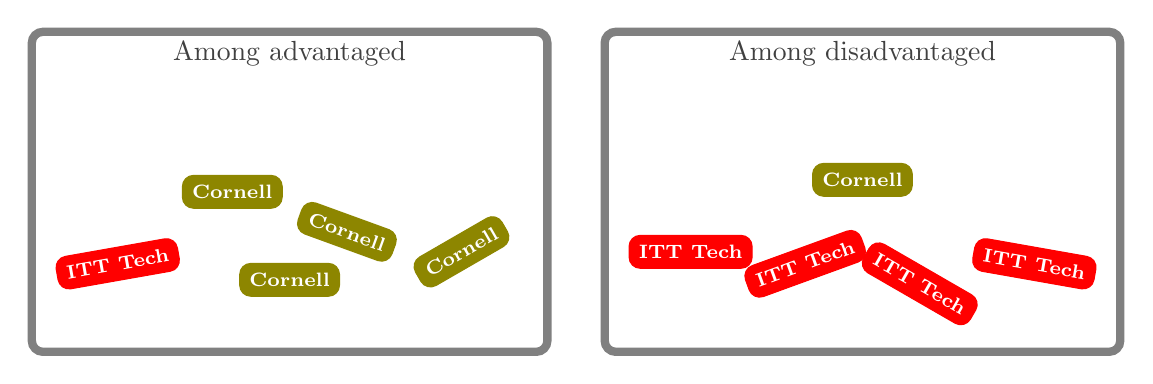
\begin{tikzpicture}[x = .6\textwidth, y = 2in]
	%% BUCKET A' %%
\draw[rounded corners, line width = 3pt, color = gray] (-.95, -.05) rectangle (-.05, .75);
\node[anchor = north, darkgray] at (-.5,.75) {{Among advantaged}};
\node[align=center, fill = olive, draw = olive, font = {\bf\scriptsize}, draw, rounded corners, inner sep = 3.5pt] at (-.5, .13) {\textcolor{white}{Cornell}};
\node[align=center, fill = red, draw = red, font = {\bf\scriptsize}, draw, rounded corners, inner sep = 3.5pt, rotate = 10] at (-.8, .17) {\textcolor{white}{ITT Tech}};
\node[align=center, fill = olive, draw = olive, font = {\bf\scriptsize}, draw, rounded corners, inner sep = 3.5pt, rotate = 30] at (-.2, .2) {\textcolor{white}{Cornell}};
\node[align=center, fill = olive, draw = olive, font = {\bf\scriptsize}, draw, rounded corners, inner sep = 3.5pt, rotate = -20] at (-.4, .25) {\textcolor{white}{Cornell}};
\node[align=center, fill = olive, draw = olive, font = {\bf\scriptsize}, draw, rounded corners, inner sep = 3.5pt] at (-.6, .35) {\textcolor{white}{Cornell}};
	%% BUCKET A %%
\pause
\draw[rounded corners, line width = 3pt, color = gray] (.95, -.05) rectangle (.05, .75);
\node[anchor = north, darkgray] at (.5,.75) {{Among disadvantaged}};
\node[align=center, fill = red, draw = red, font = {\bf\scriptsize}, draw, rounded corners, inner sep = 3.5pt, rotate = 0] at (.2, .2) {\textcolor{white}{ITT Tech}};
\node[align=center, fill = red, draw = red, font = {\bf\scriptsize}, draw, rounded corners, inner sep = 3.5pt, rotate = 20] at (.4, .17) {\textcolor{white}{ITT Tech}};
\node[align=center, fill = olive, draw = olive, font = {\bf\scriptsize}, draw, rounded corners, inner sep = 3.5pt] at (.5, .38) {\textcolor{white}{Cornell}};
\node[align=center, fill = red, draw = red, font = {\bf\scriptsize}, draw, rounded corners, inner sep = 3.5pt, rotate = -30] at (.6, .12) {\textcolor{white}{ITT Tech}};
\node[align=center, fill = red, draw = red, font = {\bf\scriptsize}, draw, rounded corners, inner sep = 3.5pt, rotate = -10] at (.8, .17) {\textcolor{white}{ITT Tech}};
\end{tikzpicture}} \\
\onslide<5->{Mistaken claim: College is more helpful to the advantaged.} \\
\onslide<6->{Better claim: The advantaged disproportionately take the effective treatment.}

\end{frame}

\begin{frame}{Multiple versions: A few resolutions}

\pause
\begin{enumerate}[<+->]
\item Assume treatment variation irrelevance
\begin{itemize}
\item If two distinct treatments (e.g., Cornell BA and Yale BA)\\map to the same treatment value in the data (BA),\\then assume they have the same effect.
\item More plausible in some settings (Cornell and Yale) than others (Cornell and ITT Tech)
\end{itemize}
\item Measure very detailed treatments
\begin{itemize}
\item Case study of Cornell degrees rather than degrees writ large
\end{itemize}
\item Study an aggregation of potential outcomes
\begin{itemize}
\item Effect of a college degree, averaged over the marginal distribution of colleges
\item Requires great care to specify the estimand here
\end{itemize}
\end{enumerate}

\end{frame}

\begin{frame}{Closing comparison}
It is nice to have two potential outcomes: $Y_i^1$ and $Y_i^0$ \pause \vskip .2in
But often the world is not so simple: \pause
\begin{itemize}
\item {\blue Interference:} Maybe the treatment is a population vector\\Example: $Y_i^{100001110}$, perhaps denoted $Y_i^{\vec{a}}$ \pause
\item {\blue Multiple versions:} Maybe the treatment is a non-binary scalar\\Example: $Y_i^{\text{Cornell}}$ $Y_i^\text{Yale}$ $Y_i^\text{Princeton}$ $Y_i^\text{ITT Tech}$ \pause
\end{itemize}
In each case, there are many more potential outcomes. \pause \vskip .2in
To collapse the potential outcomes requires theoretical argument. \vskip .3in \pause
\begin{center} \Large More research on these questions!\end{center}

\end{frame}

\goalsframe

\begin{frame}{Let me know what you are thinking}

\begin{huge} \bref{https://tinyurl.com/CausalQuestions}{tinyurl.com/CausalQuestions} \end{huge}
\vskip .7in

Office hours TTh 11am-12pm and at \bref{https://calendly.com/ianlundberg/office-hours}{calendly.com/ianlundberg/office-hours}\\Come say hi!

\end{frame}

\end{document}





